\subsection{Módulo de Administración e Inteligencia de Negocio (ADM)}

\begin{figure}[H]\centering
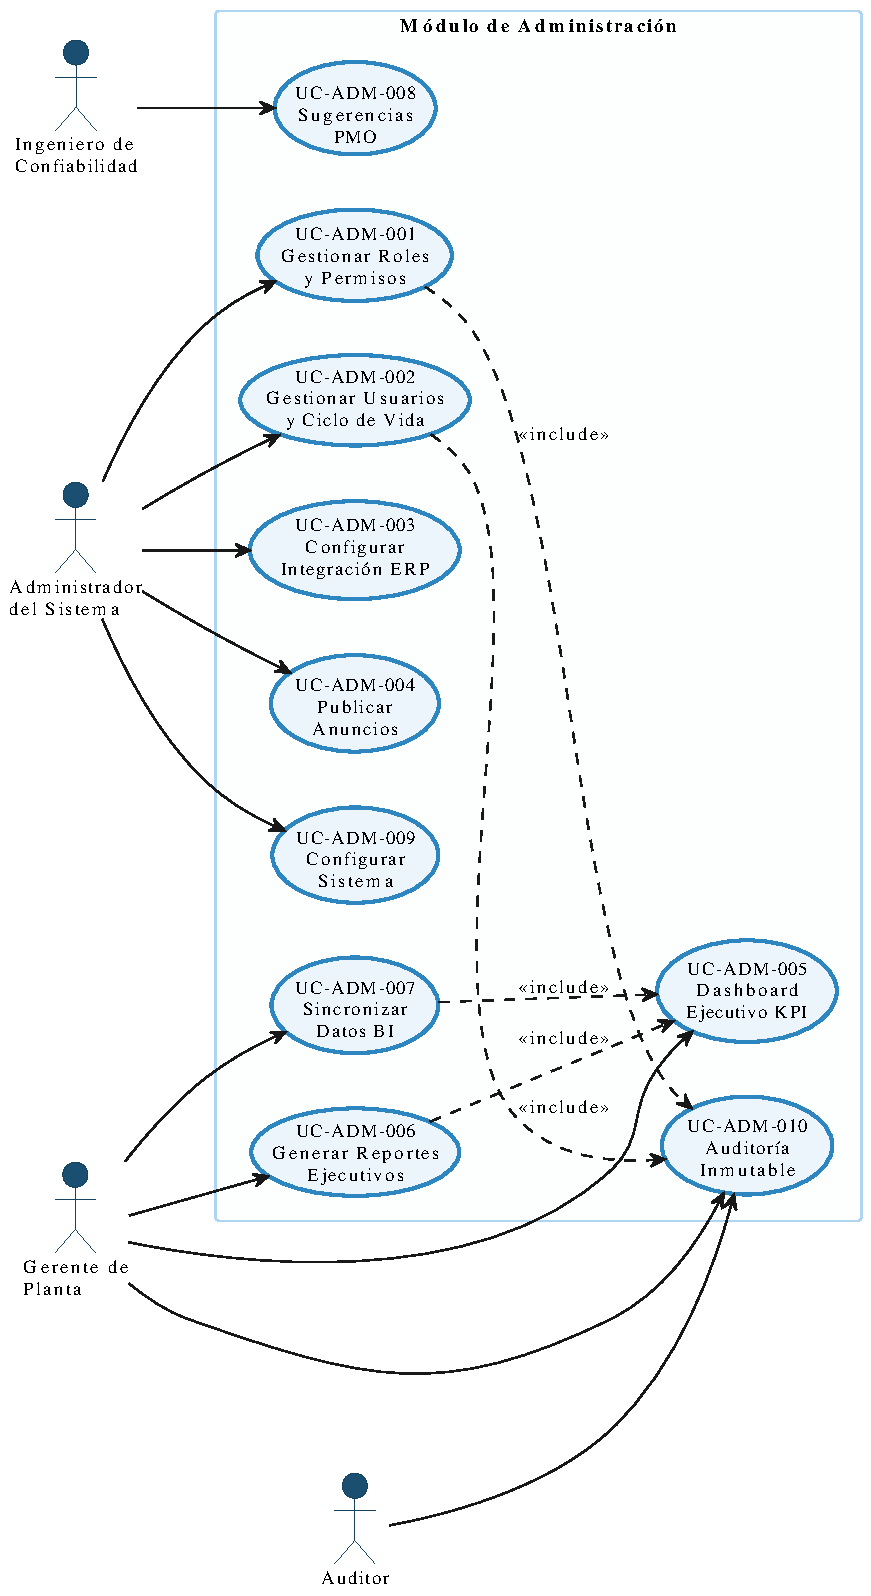
\includegraphics[width=0.85\textwidth]{assets/Diagrama-UC-ADM.pdf}
\caption{Diagrama de Casos de Uso - Administración e Inteligencia de Negocio}\end{figure}

\noindent\textbf{Ficha de Caso de Uso: UC-ADM-010 - Sistema de Auditoría Inmutable}
\footnotesize\setlength{\tabcolsep}{4pt}\renewcommand{\arraystretch}{1.2}
\rowcolors{2}{tableBlue}{white}\begin{longtable}{>{\raggedright\arraybackslash}p{0.21\textwidth} >{\raggedright\arraybackslash}p{0.74\textwidth}} \toprule
\textbf{Actor Principal} & Gerente de Planta \\
\textbf{Actores Secundarios} & Auditor, Administrador del Sistema \\
\textbf{Descripción} & Permite consultar y validar el registro cronológico e inalterable de acciones críticas para cumplimiento normativo y análisis de incidentes. \\
\textbf{Precondiciones} & \parbox[t]{\linewidth}{\vspace{2pt} \begin{itemize}[leftmargin=1.5em, nosep, topsep=0pt]
\item El usuario está autenticado con rol autorizado
\item Existen registros de auditoría disponibles
\end{itemize} \vspace{2pt}} \\
\textbf{Flujo Principal} & \parbox[t]{\linewidth}{\vspace{2pt} \begin{enumerate}[leftmargin=1.5em, nosep, topsep=0pt]
\item El Gerente accede al módulo de Auditoría y selecciona ``Consultar Registro'' (FR-348).
\item El Sistema presenta opciones de filtrado por fechas, usuario, tipo de operación y entidad (FR-348).
\item El Gerente aplica filtros y solicita la consulta.
\item El Sistema entrega resultados de la consulta con detalles resumidos (FR-349).
\item El Gerente selecciona un registro y el Sistema permite consultar el detalle completo (FR-349).
\item El Sistema valida la integridad del registro consultado y marca cualquier anomalía crítica (FR-346, FR-351, [TR-003]).
\item El Sistema registra la consulta para trazabilidad de auditoría [TR-001].
\end{enumerate} \vspace{2pt}} \\
\textbf{Flujos Alternativos} & \parbox[t]{\linewidth}{\vspace{2pt} \vspace{4pt}\noindent\textbf{AF-001: Integridad Comprometida}
\newline
En el paso 6, si se detecta anomalía:
\begin{enumerate}[leftmargin=1.5em, nosep, topsep=0pt]
\item El Sistema notifica alerta crítica y bloquea exportación del rango comprometido (FR-346).
\item El flujo se detiene y notifica al Auditor.
\end{enumerate}
\vspace{4pt}\noindent\textbf{AF-002: Rango sin resultados}
\newline
En el paso 4, si no hay registros:
\begin{enumerate}[leftmargin=1.5em, nosep, topsep=0pt]
\item El Sistema comunica el mensaje: ``No hay registros en el rango seleccionado''.
\item El flujo regresa al paso 2.
\end{enumerate} \vspace{2pt}} \\
\textbf{Postcondiciones} & \parbox[t]{\linewidth}{\vspace{2pt} \begin{itemize}[leftmargin=1.5em, nosep, topsep=0pt]
\item El usuario obtiene la trazabilidad requerida
\item Las consultas quedan registradas de forma inmutable [TR-001]
\item Cualquier anomalía queda marcada y notificada
\end{itemize} \vspace{2pt}} \\
\textbf{Requisitos} & FR-345 a FR-353 [TR-001, TR-002, TR-003] \\ \bottomrule
\end{longtable}\normalsize\vspace{1em}
\noindent\textbf{Ficha de Caso de Uso: UC-ADM-001 - Gestión de Roles y Matriz de Permisos}
\footnotesize\setlength{\tabcolsep}{4pt}\renewcommand{\arraystretch}{1.2}
\rowcolors{2}{tableBlue}{white}\begin{longtable}{>{\raggedright\arraybackslash}p{0.21\textwidth} >{\raggedright\arraybackslash}p{0.74\textwidth}} \toprule
\textbf{Actor Principal} & Administrador del Sistema \\
\textbf{Actores Secundarios} & Auditor (consulta), Supervisor HSEQ (validación SoD) \\
\textbf{Descripción} & Permite definir roles y una matriz de control de acceso basada en roles, con segregación de funciones y trazabilidad completa conforme a ISO 55001. \\
\textbf{Precondiciones} & \parbox[t]{\linewidth}{\vspace{2pt} \begin{itemize}[leftmargin=1.5em, nosep, topsep=0pt]
\item El Administrador está autenticado
\item La matriz de permisos está disponible
\end{itemize} \vspace{2pt}} \\
\textbf{Flujo Principal} & \parbox[t]{\linewidth}{\vspace{2pt} \begin{enumerate}[leftmargin=1.5em, nosep, topsep=0pt]
\item El Administrador accede al módulo de Roles y selecciona ``Crear Rol'' (FR-247).
\item El Sistema presenta formulario de creación con nombre, descripción y módulos aplicables (FR-247).
\item El Administrador define permisos en la matriz de control de acceso basada en roles (FR-248).
\item El Sistema valida reglas de segregación de funciones y solicita confirmación si hay conflicto (FR-249).
\item El Administrador confirma la creación del rol.
\item El Sistema registra el rol y la matriz de permisos en auditoría inmutable (FR-247, FR-248, [TR-001]).
\item El Sistema comunica la confirmación: ``Rol creado exitosamente''.
\end{enumerate} \vspace{2pt}} \\
\textbf{Flujos Alternativos} & \parbox[t]{\linewidth}{\vspace{2pt} \vspace{4pt}\noindent\textbf{AF-001: Conflicto de Segregación de Funciones}
\newline
En el paso 4, si se detecta conflicto:
\begin{enumerate}[leftmargin=1.5em, nosep, topsep=0pt]
\item El Sistema muestra advertencia con los permisos en conflicto (FR-249).
\item El Administrador decide ajustar o confirmar la excepción.
\item El flujo continúa en el paso 5.
\end{enumerate}
\vspace{4pt}\noindent\textbf{AF-002: Intento de modificar rol raíz}
\newline
Si el Administrador intenta modificar el rol raíz:
\begin{enumerate}[leftmargin=1.5em, nosep, topsep=0pt]
\item El Sistema bloquea la acción y muestra error crítico (FR-250).
\item El flujo termina.
\end{enumerate} \vspace{2pt}} \\
\textbf{Postcondiciones} & \parbox[t]{\linewidth}{\vspace{2pt} \begin{itemize}[leftmargin=1.5em, nosep, topsep=0pt]
\item El rol queda disponible para asignación
\item La matriz de permisos queda auditada [TR-001]
\end{itemize} \vspace{2pt}} \\
\textbf{Requisitos} & FR-247 a FR-254 [TR-001, TR-002] \\ \bottomrule
\end{longtable}\normalsize\vspace{1em}